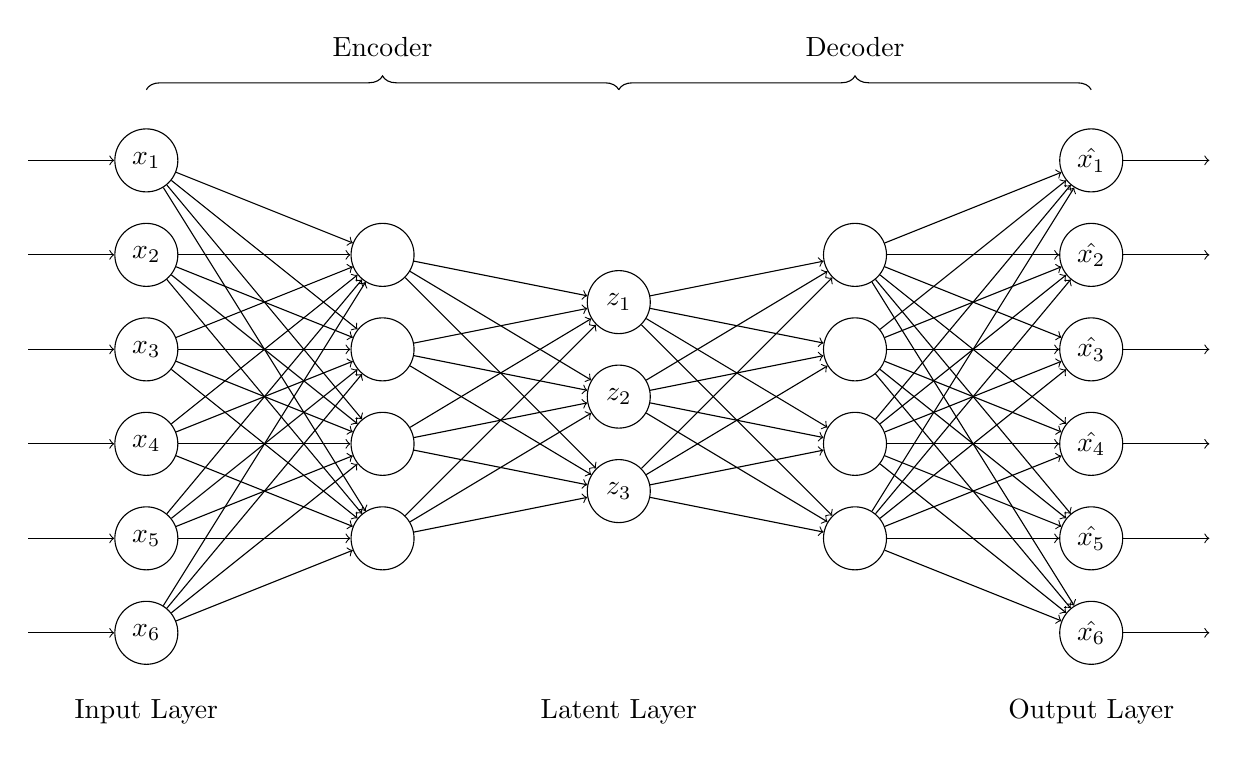
\begin{tikzpicture}
    \tikzstyle{place}=[circle, draw=black, minimum size = 8mm]

    % Input
    \foreach \x in {1,...,6}
        \draw node at (0, -\x*1.2) [place] (first_\x) {$x_\x$};

    % Hidden 1
    \foreach \x in {1,...,4}
        \node at (3, -1.2 -\x*1.2) [place] (second_\x){};

    % Latent
    \foreach \x in {1,...,3}
        \node at (6, -1.8 -\x*1.2) [place] (third_\x){$z_\x$};

    % Hidden 2
    \foreach \x in {1,...,4}
        \node at (9, -1.2 -\x*1.2) [place] (fourth_\x){};

    % Output
    \foreach \x in {1,...,6}
        \draw node at (12, -\x*1.2) [place] (fifth_\x) {$\hat{x_\x}$};
        
    \foreach \i in {1,...,6}
        \draw [->] (-1.5, -\i*1.2) to (first_\i);

    \foreach \i in {1,...,6}
        \foreach \j in {1,...,4}
        \draw [->] (first_\i) to (second_\j);

    \foreach \i in {1,...,4}
        \foreach \j in {1,...,3}
            \draw [->] (second_\i) to (third_\j);

    \foreach \i in {1,...,3}
        \foreach \j in {1,...,4}
        \draw [->] (third_\i) to (fourth_\j);

    \foreach \i in {1,...,4}
        \foreach \j in {1,...,6}
            \draw [->] (fourth_\i) to (fifth_\j);

    \foreach \i in {1,...,6}
        \draw [->] (fifth_\i) to (13.5, -\i*1.2);

    \draw [decorate,decoration={brace,amplitude=5pt,raise=-2ex}]
        (0,0) -- (6,0) node[above,midway]{Encoder};
    \draw [decorate,decoration={brace,amplitude=5pt,raise=-2ex}]
        (6,0) -- (12,0) node[above,midway]{Decoder};

    % Text
    \node at (0, -8.2) [black, ] {Input Layer};
    \node at (6, -8.2) [black, ] {Latent Layer};
    \node at (12, -8.2) [black, ] {Output Layer};
\end{tikzpicture}